\documentclass{article}
\usepackage{graphicx}
\usepackage[margin=1.5cm]{geometry}
\usepackage{amsmath}

\begin{document}

\title{Tuesday Reading Assessment: Chapter 8-1 through 8-4}
\author{Prof. Jordan C. Hanson}

\maketitle

\begin{figure}[ht]
\centering
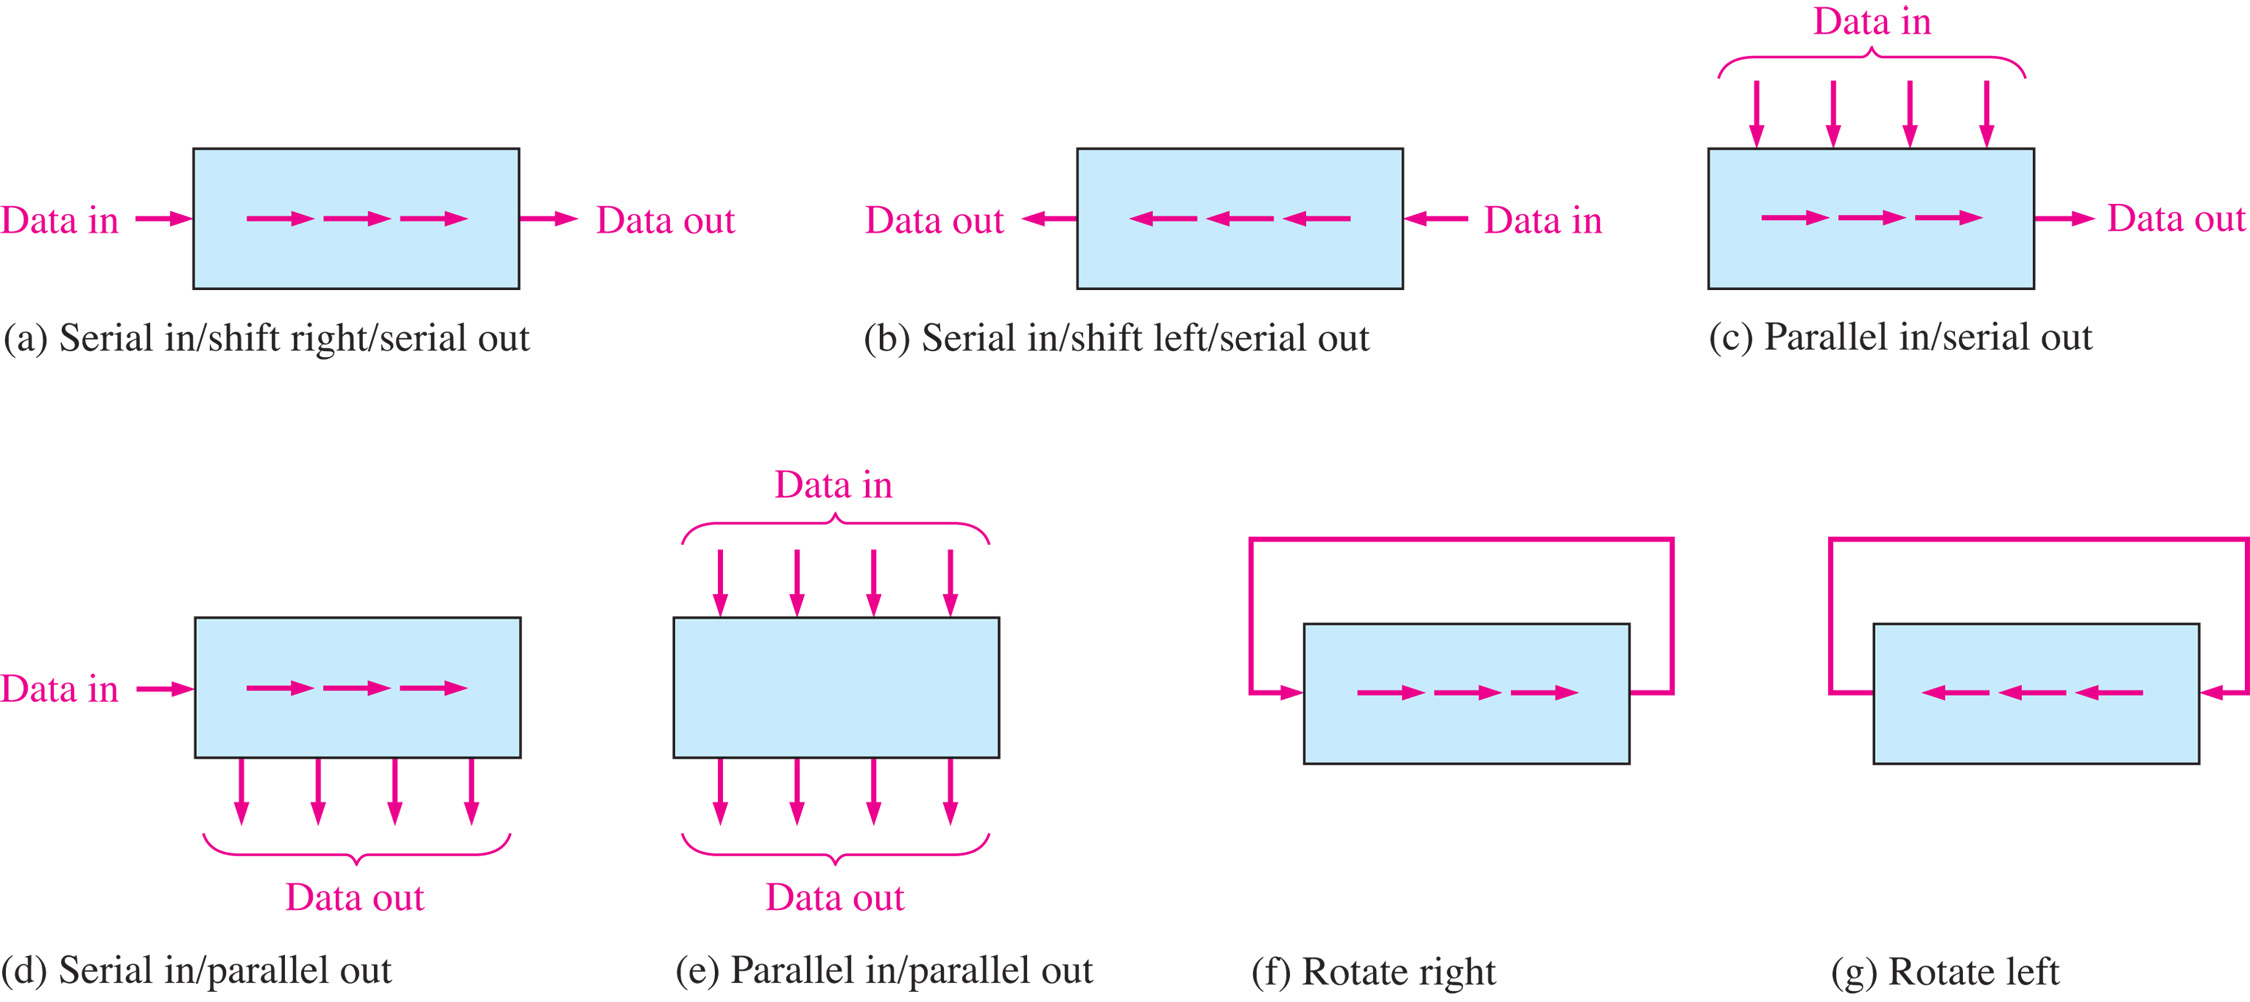
\includegraphics[width=0.75\textwidth,trim=0cm 6cm 0cm 0cm,clip=true]{figures/shift_1.jpg}
\caption{\label{fig:1} Topologies for 4-bit shift registers.}
\end{figure}

\section{Shift Registers from D Flip-Flops}

\begin{enumerate}
\item (a) Consider Fig. \ref{fig:1} (a), the 4-bit serial-in/serial-out shift register.  If the initial input is a 1, followed by 0's only, how many clock cycles before the 1 reaches the output?  Assume all flip-flops are initially reset. (b) If the clock frequency is 5 MHz, how long before the initial 1 reaches the output? (c) Consider Fig. \ref{fig:1} (c), the 4-bit parallel in/serial out shift register.  If 4 1's are on the inputs initially, how many clock cycles will pass before a 1 appears one the output? (d) If the clock frequency is 2 MHz, how long before the first 1 appears on the output? \\ \vspace{2cm}
\item (a) Consider Fig. \ref{fig:2}.  Will the data bits $D_i$ be loaded into the register when the SHIFT signal is LOW, or HIGH? (b) To shift data to the right, which two signals have to be activated, and with what values? \\ \vspace{1cm}
\end{enumerate}

\begin{figure}[hb]
\centering
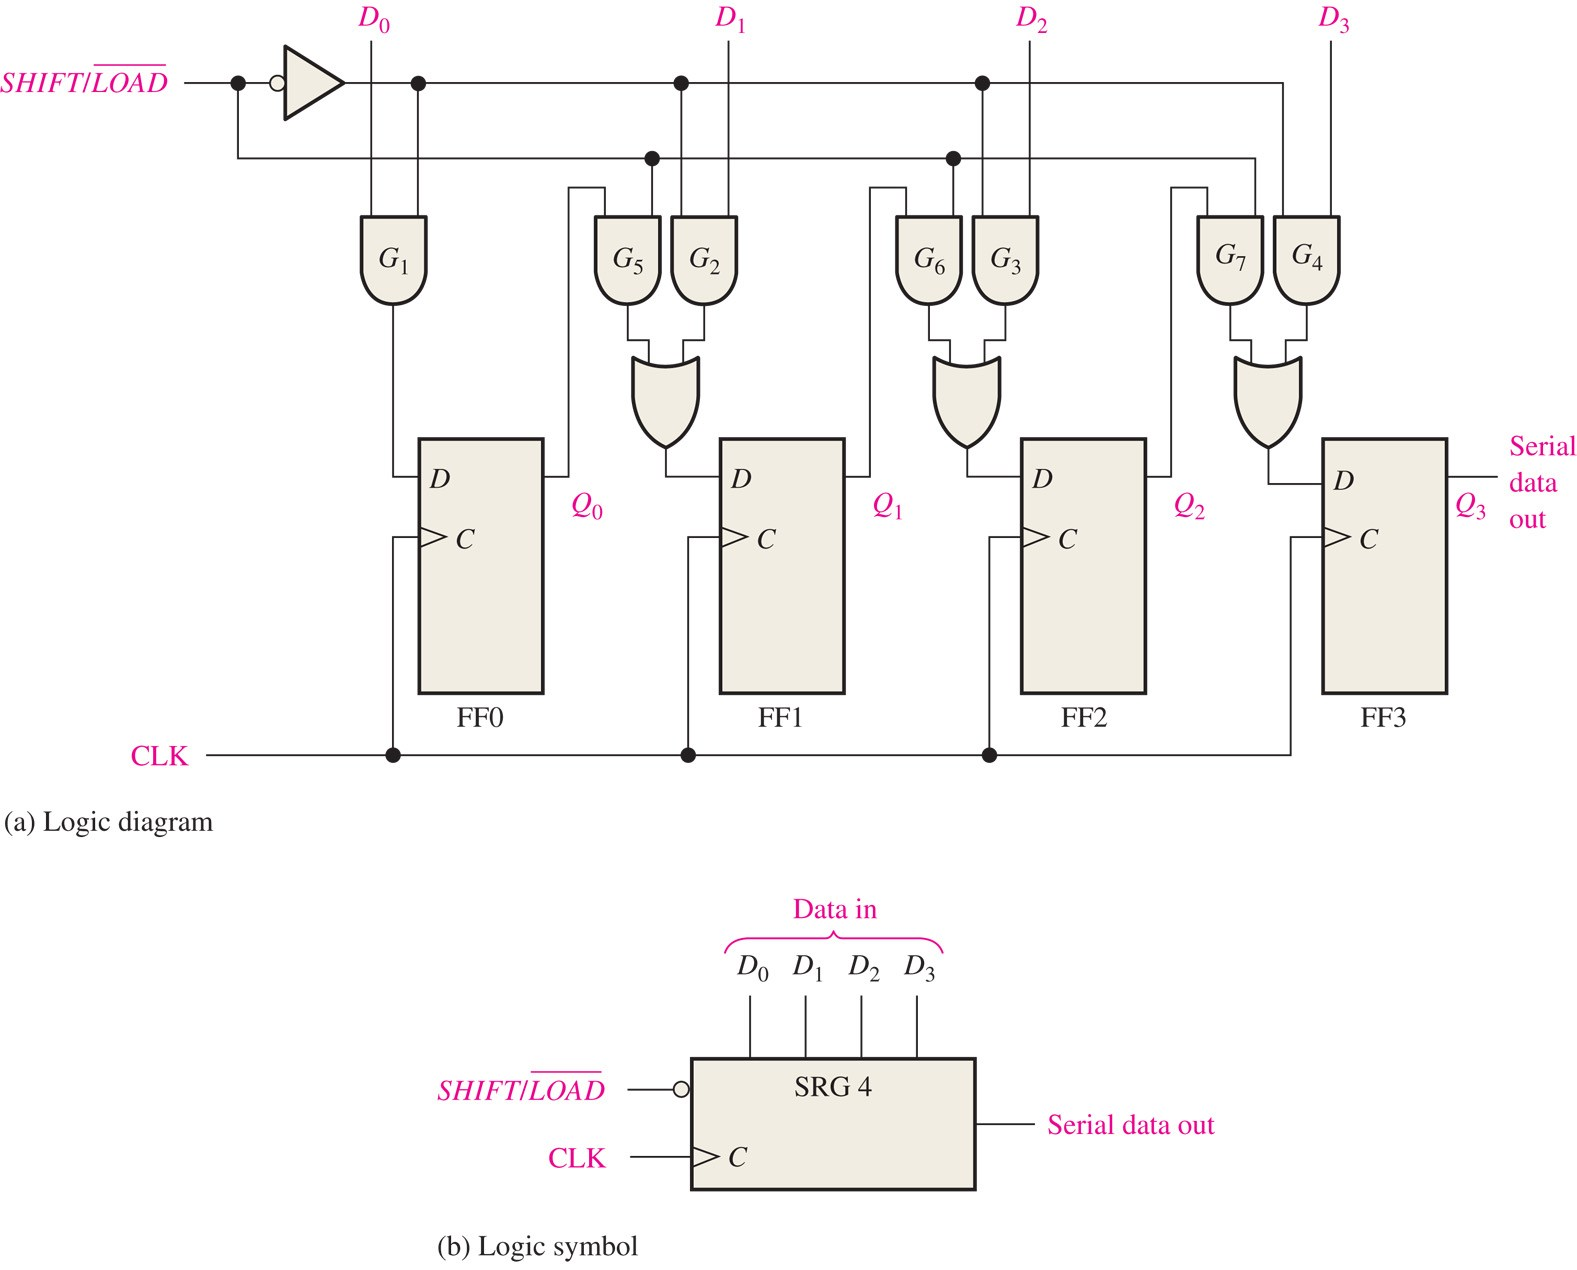
\includegraphics[width=0.6\textwidth,trim=0cm 5cm 0cm 0cm,clip=true]{figures/shift_2.jpg}
\caption{\label{fig:2} A 4-bit parallel-in/serial out shift register.}
\end{figure}

\end{document}
